\mysubsection{Positionnement des robots}
Une fois que les robots ont été déjà choisi, la deuxième étape consiste à déterminer le positionnement des robots par rapport aux fournitures, dont positions ont été déjà fourni dans la consigne de l’avant projet (ou dans un cas réel, cela représente le vrai positionnement des fournitures ou des machines dans l’usine).\\

Premièrement, comme les convoyeurs des caisses ont une hauteur de 1085 mm et le rayon de travail des robots qui vont remplir les caisses est 911 mm, on a besoin d’utiliser un piédestal pour eux. On sait bien qu’utiliser un piédestal ajoute des frais au projet, et à mesure que la hauteur du piédestal augmente, son prix augmente aussi. Donc on doit choisir le piédestal le plus bas qui permet au robot de bien réaliser ses activités, afin de réduire les frais. Ce choix implique une analyse de toutes les tailles de piédestal disponible dans le marché et leur prix, qu’on n’a pas trouvé, et il y a une relation aussi avec la distance horizontale entre le robot et le convoyeur. Empiriquement, on doit choisir un piédestal un peu plus bas que le convoyeur (environ 1000 mm de hauteur). La distance horizontale par rapport au point le plus loin qu’il doit placer une bouteille doit être inférieure, au moins de 50 mm, au rayon de travail du robot (861 mm). Dans la solution de l’avant-projet, ils ont choisi une hauteur de 1100 mm et une distance horizontale d’environ 775 mm. 

Pour le robot de palettisation, une fois qu’on doit palettiser 9 couches de caisses sur une palette qui est sur un convoyeur totalisant 3023.5 mm de hauteur et le rayon de travail du robot est de 2655 mm, on a besoin aussi d’un piédestal. En considérant que les caisses doivent être empilés pour la haute et que la distance entre les caisses remplies dans le convoyeur et la position la plus loin dans la palette est d’environ 1200 mm, le piédestal doit avoir au minimum 1000 mm. Ils ont choisi une hauteur de 1400 mm, et le robot est placé d’une façon équidistant entre le convoyeur de caisses et le point le plus loin de la palette qui est remplie. 

Peut-être s’ils avaient choisi des piédestal plus bas pour les trois robots, ils seraient arrivés dans uns solution moins chère et qui marche aussi bien. Pour avoir une solution optimale dans ce cas-là, on a besoin de simuler le programme en augmentant les hauteurs des piédestal. Mais pour le positionnement horizontale des robots, nous sommes complètement d’accord avec ce qui a été fait.

\mysubsection{Mouvement des robots}
Pour finir tous les éléments de la simulation, on doit ajouter aussi la laveuse / sécheuse, les grillages de sécurité et un contrôleur pour les trois robots. Placer le contrôleur dehors de la zone de sécurité facilite beaucoup le fonctionnement de la cellule pour éviter que les personnes rentrent dans la zone de sécurité. L’image \ref{fig:rap3} montre la cellule robotique.

\begin{figure}[H]
	\begin{center}	
		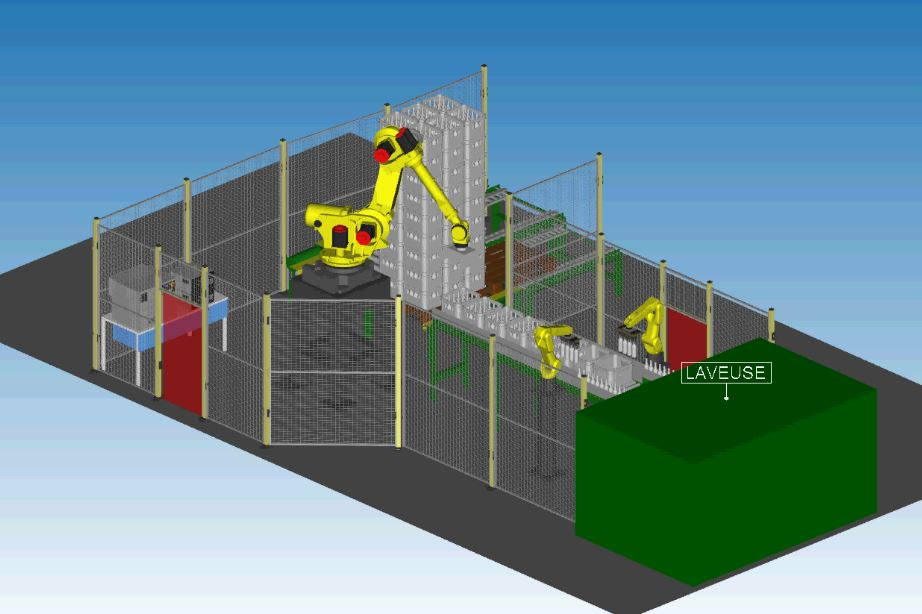
\includegraphics[width=8cm]{./rap3.JPG}
		\caption{La cellule robotique.}
		\label{fig:rap3}
	\end{center}
\end{figure}

Ensuite, on doit choisir les trajectoires des robots. Pour les robots des caisses, on doit se rassurer que les bouteilles sont mises par la haute et qu’elles ne vont pas frapper d’autres objets. Pour cela, on rajoute un point CNT100 au début du convoyeur et un point CNT10 sur la position voulue pour les bouteilles, dans une hauteur de 600 mm (caisse + bouteille) par rapport au convoyeur, et un point FINE dans la position voulue (cette position et la dernière position de rapproche vont changer avec un offset pour correctement remplir la caisse de cinq lignes de quatre bouteilles). On peut utiliser les mouvements JOINT pour les robots, qui sont plus rapides et suffisant dans ce cas. Les trajectoires sont illustrées dans la figure \ref{fig:rap1}. C’est convenable d’aligner les robots, la caisse et les quatre bouteilles avant de les prendre, en arrêtant le convoyeur de caisses dans cette position.

\begin{figure}[H]
	\begin{center}	
		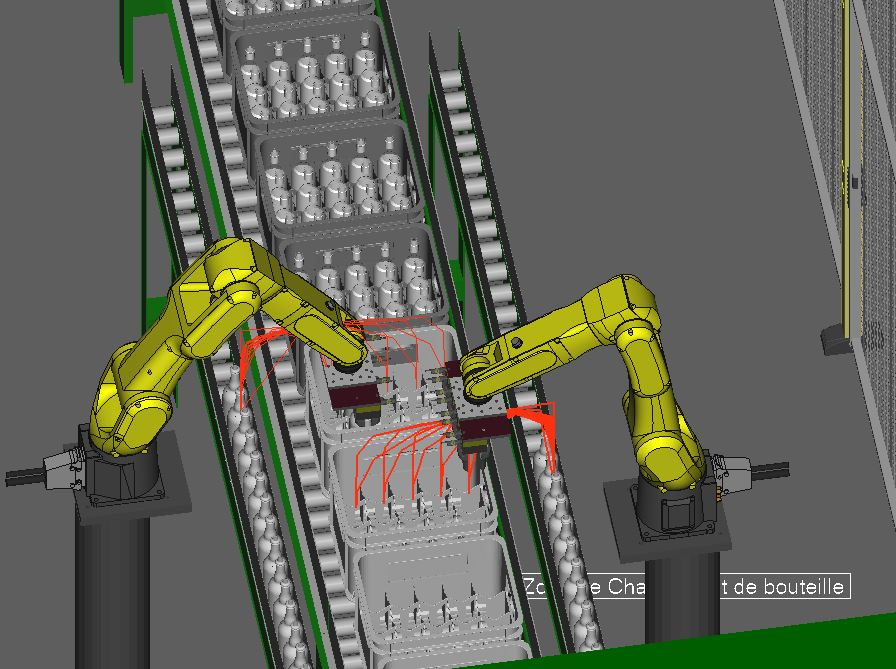
\includegraphics[width=8cm]{./rap1.JPG}
		\caption{Procès de remplissage des caisses.}
		\label{fig:rap1}
	\end{center}
\end{figure}

On peut utiliser la même idée pour générer le mouvement du robot de palettisation, sauf que pour lui, on va avoir besoin d’utiliser l’offset dans tous les axes (X, Y et Z) pour les trois points (les deux points de rapproche et le point de dépose). Ce robot doit empilé deux caisses dans les palettes avant que les autres finissent de les remplir pour que le convoyeur puisse bien marcher. La figure \ref{fig:rap2} illustre la trajectoire de ce robot.

\begin{figure}[H]
	\begin{center}	
		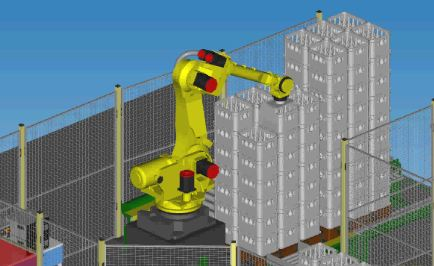
\includegraphics[width=8cm]{./rap2.JPG}
		\caption{Procès de palettisation.}
		\label{fig:rap2}
	\end{center}
\end{figure}

Pour finir, on peut ajouter des éléments DCS dans cette cellule, qui ne sont pas vraiment nécessaires dans ce cas, mais c’est toujours bien de les mettre dans une cellule robotique. Comme la probabilité d’avoir une personne dans la zone de sécurité est faible, on peut simplement éteindre les robots lorsqu’il y a une personne dans cette zone (probablement pour la maintenance des robots et des machines).





